%\documentclass[tikz,14pt,russian]{standalone}
% Third parameter is needed for TOC displaying (why?)
\usepackage{../common/dsturep} % оформление по ДСТУ 3008-95
\usepackage{import}
\usepackage{standalone}
\usepackage{comment}
\usepackage{bbm}

\usepackage{tikz}
\usepackage{tikz-3dplot}
\usetikzlibrary{calc}
\usetikzlibrary{plotmarks}
\usepackage{pgfplots}

%\usepackage{scrextend}
\usepackage{changepage}
\usepackage{caption}
\usepackage{listings}
%\usepackage[title,titletoc]{appendix}
%\usepackage{appendix}
\usepackage{longtable}
%\usepackage{slashbox}
\usepackage{diagbox}
\usepackage{lscape}
\usepackage{algorithmic}
\usepackage{algorithm}

\newcommand{\indicatorof}[1]{\mathbbm{1}_{#1}}
\newcommand{\indicator}[1]{\mathbbm{1}\!\left( #1 \right)}
\newcommand{\Indicator}[1]{\mathbbm{1}\!\left\{ #1 \right\}}
\newcommand{\probability}[1]{\mathbb{P}\left( #1 \right)}
\newcommand{\Probability}[1]{\mathbb{P}\left\{ #1 \right\}}
\newcommand{\cdfof}[2]{F^{#1}\left(#2\right)}
\newcommand{\cdf}[1]{\cdfof{}{#1}}
\def\Tau{\mathrm{T}}
\newcommand{\meanof}[2]{\operatorname{M}_{#1} #2}
\newcommand{\Meanof}[2]{\meanof{#1}{\left[ #2 \right]}}
\newcommand{\mean}[1]{\meanof{}{#1}}
\newcommand{\Mean}[1]{\Meanof{}{#1}}
\newcommand{\dispersionof}[2]{\operatorname{D}_{#1} #2}
\newcommand{\Dispersionof}[2]{\dispersionof{#1}{\left[ #2 \right]}}
\newcommand{\dispersion}[1]{\dispersionof{}{#1}}
\def \mcond {\;\middle|\;}
\newcommand{\Covergencen}[1]{\xrightarrow[#1\to\infty]{}}
\newcommand{\cov}[1]{\operatorname{cov}\!\left( #1 \right)}
\DeclareMathOperator*{\argmax}{arg\,max}
\DeclareMathOperator*{\argmin}{arg\,min}

\newcommand{\drawHist}[1]{\begin{tikzpicture}[scale=1]
  \begin{axis}[ymin=-5, ymax=5, xmin=5, xmax=30, ytick=\empty,
    xmajorgrids={true},
    ylabel={Кількість точок}, ylabel near ticks,
    xlabel={час, с}]

\draw[dashed,color=gray!50] ({rel axis cs:0,0}|-{axis cs:0,0}) -- ({rel axis cs:1,0}|-{axis cs:0,0});
\addplot table [x, y, col sep=comma] {data/#1.csv};
\end{axis}
\end{tikzpicture}}

\captionsetup[subfigure]{skip=0ex} % global setting for subfigure

\usepackage{stringenc}
\usepackage{pdfescape}

\makeatletter
\renewcommand*{\UTFviii@defined}[1]{%
  \ifx#1\relax
    \begingroup
      % Remove prefix "\u8:"
      \def\x##1:{}%
      % Extract Unicode char from command name
      % (utf8.def does not support surrogates)
      \edef\x{\expandafter\x\string#1}%
      \StringEncodingConvert\x\x{utf8}{utf16be}% convert to UTF-16BE
      % Hexadecimal representation
      \EdefEscapeHex\x\x
      % Enhanced error message
      \PackageError{inputenc}{Unicode\space char\space \string#1\space
                              (U+\x)\MessageBreak
                              not\space set\space up\space
                              for\space use\space with\space LaTeX}\@eha
    \endgroup
  \else\expandafter
    #1%
  \fi
}
\makeatother
\DeclareUnicodeCharacter{00AD}{-}

\def\male{male}
\def\female{female}

%\input{../common/minted.inc}   % оформление листингов в minted
%\bibliographystyle{../common/utf8gost705u}
%\bibliographystyle{../common/utf8gost71u}
\bibliographystyle{../common/utf8gost780u}
%\bibliographystyle{plain}

\usepackage[square,numbers,sort&compress]{natbib}
\renewcommand{\bibnumfmt}[1]{#1.\hfill} % нумерация источников в самом списке — через точку
%\renewcommand{\bibsection}

\usepackage{glossaries}
\makeglossaries


\begin{document}

\fancypagestyle{firststyle}
{
    \fancyfoot[C]{Київ --- \passYear~року}
    \fancyhead{}
}
\begin{titlepage}
  \thispagestyle{firststyle}
  \begin{center}
      \MakeUppercase{\textbf{національний технічний університет україни}}\\[-0.5ex]
      \MakeUppercase{\textbf{``київський політехнічний інститут''}}\\[-0.5ex]
      \MakeUppercase{\textbf{\faculty}}\\
      \MakeUppercase{\department}
  \end{center}
  \begin{adjustwidth}{21em}{1em}
    \begin{flushright}
    <<До захисту допущено>>\\
    Завідувач кафедри\\
    $\underset{\text{\textit{\tiny(підпис)}}}
    {\text{\underline{\phantom{(підпис)}}}}$
    $\underset{\text{\textit{\tiny(ініціали, прізвище)}}}
    {\text{\underline{\departmentHead}}}$\\
    ``${\text{\underline{\hspace{2em}}}}$''
    ${\text{\underline{\hspace{6em}}}}$
    \passYear~р.
    \end{flushright}
  \end{adjustwidth}
  \begin{center}
      \textbf{\Large \kind }\\[1ex]
      освітньо-кваліфікаційного рівня ``\level''\\[1ex]
  \end{center}
  за спеціальністю \specialityCode~<<\specialityTitle>>\\
  на тему <<\theme>>\\
  \ifx\gender\male
    Виконав студент
  \else
    Виконала студентка
  \fi
  \course~курсу групи \group\\
  \name
  \hfill$\underset{\text{\textit{\tiny(підпис)}}}
  {\text{\underline{\phantom{(підпис)}}}}$\\
  Керівник
  \mentorRank,
  \mentorName
  \hfill$\underset{\text{\textit{\tiny(підпис)}}}
  {\text{\underline{\phantom{(підпис)}}}}$\\
  Рецензент
  \reviewerRank,
  \reviewerName
  \hfill$\underset{\text{\textit{\tiny(підпис)}}}
  {\text{\underline{\phantom{(підпис)}}}}$\\

  \begin{adjustwidth}{16em}{1em}
    Засвідчую, що у цій дипломній роботі
    немає запозичень з праць інших
    авторів без відповідних посилань.\\
    \ifx\gender\male
      Студент
    \else
      Студентка
    \fi
    \underline{\phantom{(підпис)}}
  \end{adjustwidth}

\end{titlepage}


\clearpage
\setcounter{page}{2}

%\pagestyle{empty}
\tableofcontents
\thispagestyle{empty}

\clearpage
\pagestyle{fancy}

\clearpage

%Машинне навчання\newglossaryentry{computer}

\newglossaryentry{abstraction}{
name={Абстракція},
description={узагальнення більш простих понять до більш
складних, розглядання конкретного явища замість видів, в яких воно може
поставати}
}

\newglossaryentry{machinelearning}{
name={Машинне навчання},
description={підрозділ штучного інтелекту, що вивчає методи побудови моделей,
що здатні до самонавчання}
}

\newglossaryentry{computerstudy}{
name={Комп’ютерне навчання},
description={Навчання людей за допомогою комп’ютера}
}

\newglossaryentry{expertsystem}{
name={Експертна система},
description={Комп’ютерна система, що здатна частково замінити експерта}
}

\newcommand{\textgreek}[1]{\begingroup\fontencoding{LGR}\selectfont#1\endgroup}
\newglossaryentry{ergonomics}{
name={Ергономіка},
description={(від давньогрецького \textgreek{'ergos} --- праця і
\textgreek{n'omos} --- закон) наука, про пристосування робочого місця
(зокрема комп’ютерного) для забезпечення найбільшого комфорту, ефективності
і безпеки}
}

\newglossaryentry{precedence}{
name={Прецедент},
description={специфікація послідовності дій при проектуванні програмних систем}
}

\newglossaryentry{bpmn}{
name={BPMN},
description={(з англійської Business Process Model and Notation, нотація та
модель бізнес-процесів) система умовних позначень для моделювання
бізнес-процесів}
}

\newglossaryentry{}{
name={},
description={}
}

%\newglossaryentry{}{
%name={},
%description={}
%}

\glsaddall
\addcontentsline{toc}{chapter}{Перелік термінів та умовних позначень}
\printglossary[title=Перелік термінів та умовних позначень,nonumberlist=true]

\chapter*{Вступ}
\addcontentsline{toc}{chapter}{Вступ}
% Preface template:
% \textit{Об’єкт дослідження}:

% \textit{Предмет дослідження}:

% \textit{Метою роботи є}

\textit{Об’єкт дослідження}:
користувачі, \glslink{expertsystem}{експертні системи}, їх взаємодія.

\textit{Предмет дослідження}:
поведінка користувачів при навчанні, реакція на різноманітний зовнішній вплив.

Окремий інтерес собою являє правильність трактування даних, що отримуються від
користувачів в результаті взаємодії з експертною системою, --- важливіша і
складніша частина роботи, що і відрізняє її від аналогів.

Також буде розглядатися питання
%\glslink{ergonomics}{ергономіки}
ергономіки інтерфейсу системи для найбільш ефективного процесу навчання.

\textit{Метою роботи є}
побудова експертної системи \glslink{computerstudy}{комп’ютерного навчання}
користувачів на прикладі обробки геоінформаційних даних.
Така задача є достатньо багатогранною, для її втілення потрібно працювати
з даними різного походження, також природньо виникає потреба використання
розподіленої системи.
На такій базі буде розроблено достатньо загальний метод навчання,
що використовуватиметься для інших дисциплін.

Основна задача --- мінімізувати витрати часу експерта (викладача) на процес
перевірки знань користувачів (студентів) та надання їм навчальних матеріалів,
підвищення об’єктивності оцінювання користувачів, а також оцінка роботи
самих викладачів.
Це буде зроблено шляхом розробки експертної системи, що буде аналізувати дії
користувачів, класифікувати їх, робити відповідні висновки.

Тут постає питання інформаційної безпеки, адже потрібно контролювати
користувачів --- перевіряти, чи та людина сидить за своїм робочим місцем,
запобігати списування, гарантувати максимальну безпеку базі даних з
результатами робіт, а також стежити за тим, щоб користувачі отримували коректні
завдання, а розв’язки відправлялися системі в незміненому вигляді.


\chapter{Індивідуальне завдання}
\section{Власне, завдання}
Як вже було описано вище, індивідуальне завдання --- створення розподіленої
геоінформаційної системи, призначення якої --- навчання обробці і використанню
даних, що з’являються в таких системах.
Це є векторні, растрові дані, таблиці, текстова інформація, числа, діаграми
і таке інше.
Тобто, дані мають різноманітне походження, потребують застосування різних
методів зберігання та обробки, але треба створити єдину систему, що буде
дозволяти коректно працювати з усіма даними єдиним способом.
Далі ця система буде розширена і узагальнена на інші галузі і інші потреби
--- не тільки навчання студентів, але й навчання та підвищення кваліфікації
персоналу підприємств, і не тільки для використання та обробки геоданих.

\section{Актуальність проблеми, аналоги}
В світі інформаційних технологій жити стає дуже зручно.
Завдяки потужним комп’ютерам і мережі Інтернет стає можливою передача великих
обсягів інформації за відносно малий час.
Чому б не використати можливості сучасних інформаційних технологій для більшого
покращення процесу навчання?

Перші кроки вже зроблено --- існують електронні щоденники шкільників,
електронні конспекти з різних дисциплін, електронні тести для перевірки знань.
На мою думку, найбільш розвиненою з таких систем є Coursera, що надає доступ
до навчальних матеріалів (відеолекцій, друкованих конспектів), проводить
перевірку знань у вигляді тестів. Зокрема Coursera має дуже цікаву можливість
підтвердження особистості за допомогою веб-камери та електронного почерку, що
дозволяє видавати сертифікати за проходження курсів, яким можна довіряти.

\section{Прецеденти}

\subsection{Реальне життя}

Послідовність дій студента за курс навчання якогось предмету можна розкласти
на наступні етапи:
\begin{enumerate}
    \item
        Записатися на курс (вступити до університету)
    \item\label{item:learnTheory}
        Ознайомитися з теорією (слухати лекції)
    \item\label{item:doExercises}
        Виконати практичні завдання для закріплення теорії
        (виконання домашніх завдань, контрольних робіт)
    \item
        Повторювати \ref{item:learnTheory} і \ref{item:doExercises} за
        навчальним планом
    \item
        Продемонструвати свої знання та навички у зазначений строк
        (залік, екзамен, курсова)
\end{enumerate}

Послідовність дій викладача
\begin{enumerate}
    \item
        Стати викладачем
    \item
        Створити план курсу --- лекцій, практичних занять тощо
    \item
\end{enumerate}


\chapter{Огляд літературних джерел}
Одним з найбільш повних джерел за тематикою автоматизації комп’ютерного навчання
є книга Булигіна В.Г. ``Основы автоматизации процесса обучения'' \cite{Bulygin}.
В ній досить повно розглядається проблема автоматизації навчання ---
від математичних моделей окремих компонент до фізичної реалізації цілої
загальнодержавної системи, мета якої --- покращення якості навчання взагалі.
Тим не менш, система, якій присвячено даний звіт, є складною, і необхідні для її
створення знання виходять за межі книги, хоч і переслідує все ту ж мету ---
покращення і автоматизація процессу навчання.
Наприклад, задачі створення рекомендацій для викладача, аналізу практичних робіт
студентів на предмет нечесної здачі тощо, є важливими, але так і не були
висвітлені в книзі.

Після поверхневого огляду задач системи та методів, якими вони повинні
розв’язуватись, було виділено наступні галузі знань, які потрібно більш детально
розібрати для досягнення поставленої мети:

\begin{enumerate}
    \item
        \textbf{Математичні методи прийняття рішень} для багатокритеріальних
        альтернатив.
        Дана галузь охоплює задачу вибору відповідних завдань для
        конкретного студента з урахуванням багатьох критеріїв, кількість яких
        може змінюватись як в рамках конкретного завдання, так і в залежності
        від даних, які є для конкретного студента.
        Наприклад, якщо студент вже виконував задачу $n$, то система повинна
        знайти для нього інше завдання, аби підвисити об’єктивніть оцінювання.

        Основним джерелом за темою прийняття рішень на момент написання звіту
        є курс Смірнова С.А. ``Моделі та методи прийняття рішень'', що дав
        базове бачення предметної області.
    \item
        \textbf{Методи машинного навчання} в реалізації системи необхідні для
        аналізу результатів завдань і створення необхідних рекомендацій щодо
        покращення рівня навчання. Планується аналізувати як користувачів
        (успішність та ступінь чесності студентів, об’єктивність оцінювання
        перевіряючих осіб), так і складність самих тестових завдань,
        щоб зробити оцінювання якомога більш об’єктивним.

        Для ознайомлення з деякими методами були використані матеріали ІКД
        для внутришнього користування та інформація з сайту MachineLearning.Ru
        \cite{Machinelearning}.
        Дана тема потребує більш детального вивчення перед тим, як будуть
        обрані конкретні методи та алгоритми машинного навчання.

        Під час проходження практики особливу увагу було приділено алгоритмам
        кластерізації k-means та k-means++, в задачі обробки супутникових
        знімків. Були використані як вже готові готові реалізації даних
        алгоритмів в середовищі MatLab, так і окремі реалізації, розроблені
        спеціально для задачі обробки супутникових знімків.
    \item
        \textbf{Безпека розподілених систем} займає важливе місце в даній
        роботі, адже сама система є розподіленою і передбачає використання
        декількох серверів для залучення різноманітних тестових даних.
        Також серед студентів можуть бути особи, що можуть спробувати нечесно
        змінити свої результати, знищити дані або систему, що змусить
        витратити додатковий час на відновлення системи, заново проводити
        тестування, а в крайньому разі унеможливить подальше використання
        системи за призначенням.
\end{enumerate}


\chapter{Теоретичні відомості про метод розв’язання, його обґрунтування}
Основа реалізації проекту --- розподілена експертна система.
Зрозуміло, що для цього потрібно використовувати мови програмування,
які дозволяють зручно працювати з розподіленими системами,
а також мають якомога кращу підтримку експертних систем --- готові фреймворки,
бібліотеки.

Увагу зачепили дві мови --- Erlang і Scala, коротке представлення про які
наведено далі.

\section{Erlang}
Erlang --- перевірена часом мова програмування, що була створена у 1986 році,
і розвивається до наших днів.
Створений компанією Ericsson спеціально для розподілених систем з великим
навантаженням.
Якщо в інших мовах для підтримки багатопотоковості потрібно завантаження
спеціальних бібліотек, Erlang має ці можливості як основні --- на рівні мови.

Основа розподіленої роботи в Erlang --- обмін повідомленнями між програмами, що
дозволяє розподіляти обробку даних як між різними процесами в межах одного
комп’ютеру, так між різними серверами, полегшується обробка виключних ситуацій
тощо.

Одним з фреймворків для створення експертних систем є ERESYE --- ERlang Expert
SYstem Engine (движок для створення експертних систем на Erlang) \cite{ERESYE}.

ERESYE --- це бібліотека для створення, виконання та управління машинами
виведення \cite{ErlangES}, що й треба для створення експертних систем.

\section{Scala}
Одним з варіантів платформи реалізації описуваної системи є мова програмування
Scala і відповідно віртуальна машина JVM.
Переваги використання цього варіанту:

\begin{enumerate}
    \item 
        Великий вибір готових бібліотек та можливість виконуватись будь-де (дану
        можливість реалізує платформа JVM).
    \item
        Широкий вибір програмного інструментарію для розробки розподілених
        програм.
    \item
        Наявність багатьох готових фреймворків для реалізації експертних систем,
        серед яких:
        \begin{enumerate}
            \item Drools \cite{Drools} --- перевірена часом бібліотека, що має
                відкритий програмний код та велику спільноту розробників,
                що дозволяє швидко знайти відповідь на будь-яке питання її
                стосовно функціональності.
            \item
                D3web \cite{D3web} --- більш проста бібліотека зі своїм
                Wiki-ресурсом та наявністю юніт-тестування.
                Більш просте рішення, яке, можливо, краще підходить для рішення
                задачі, описаної в даному звіті.
            \item
                jColibri \cite{jColibri} --- бібліотека, яка призначена для
                інтерактивного пошуку по великому числу варіантів.
        \end{enumerate}
\end{enumerate}

З вищенаписаного можна зробити висновок, що Scala чудово підходить для
реалізації ідей, описаних в наступному підрозділі.


\chapter{Програмна реалізація розроблених алгоритмів}
Оскільки часу було замало, а ідея нова, програмної реалізації ще немає.
Замість цього в даному розділі буде наведено основні ідеї та діаграми.

У підрозділі \ref{section:precedences} можна побачити послідовності дій
студентів та викладачів у реальному житті.
Задача даної частини доповіді --- представлення архітектури майбутньої системи.

Розглянему діаграму на рис. \ref{fig:scheme_main}, на якій представлено загальну
структуру системи --- її компоненти та зв’язки між ними.

\begin{figure}[htbp]
    \center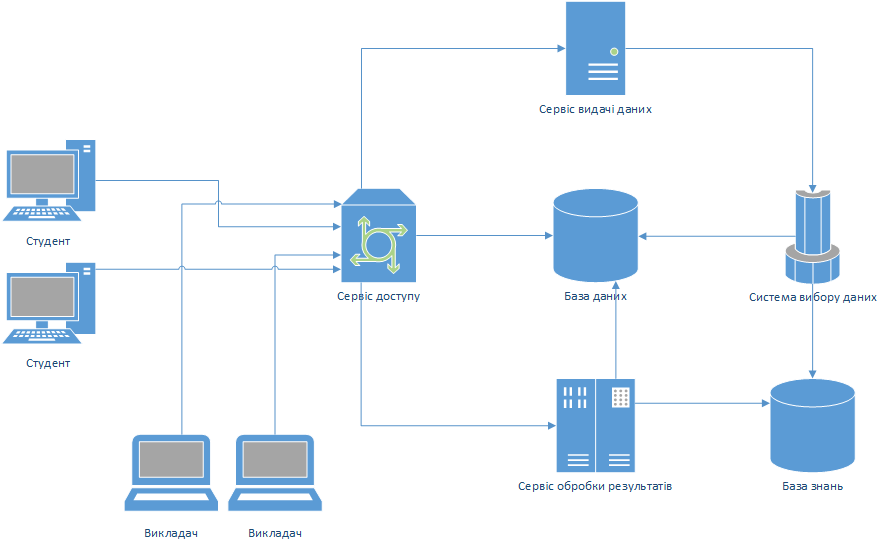
\includegraphics[width=\textwidth]{images/scheme_main.png}
    \caption{Схема роботи системи}
    \label{fig:scheme_main}
\end{figure}

Тепер подивимось на схему на рис. \ref{fig:bpmn_tests}.

\begin{figure}[h!]
    %\center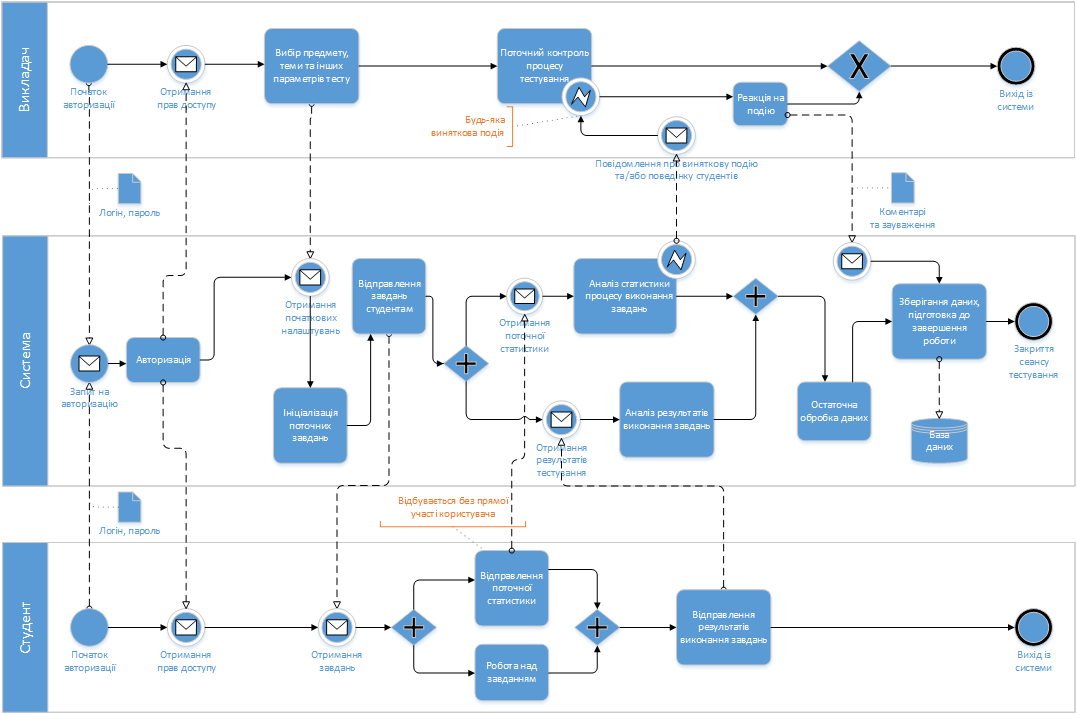
\includegraphics[height=23em,angle=90]{images/bpmn_tests.png}
    %\center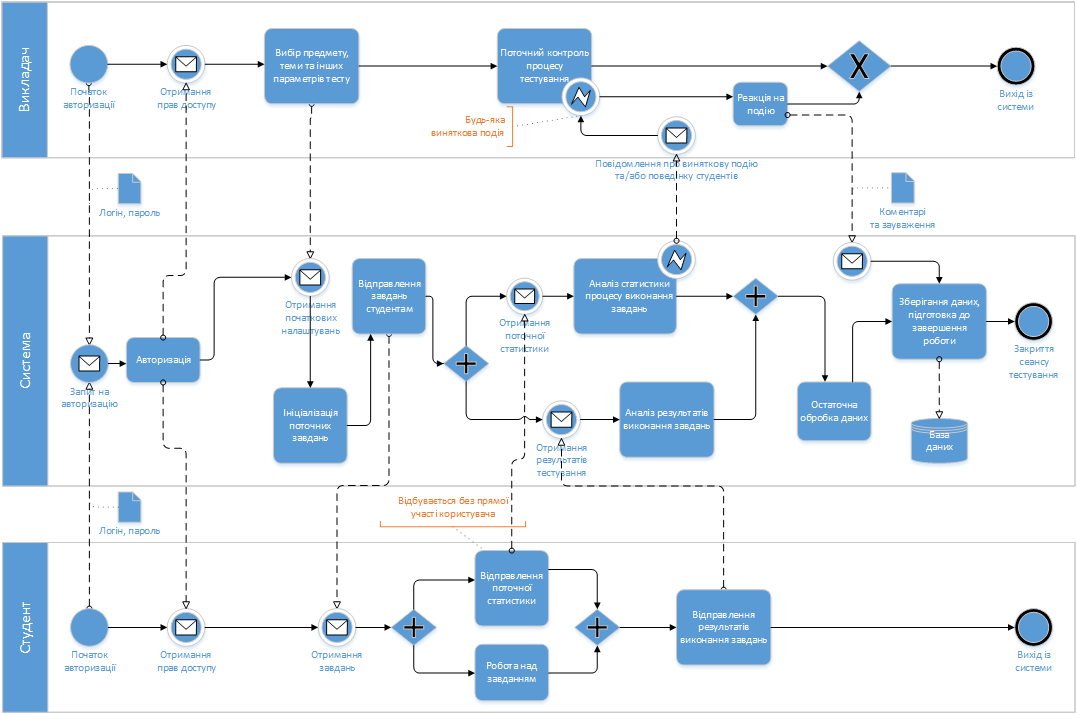
\includegraphics[width=\textwidth]{images/bpmn_tests.png}
    \center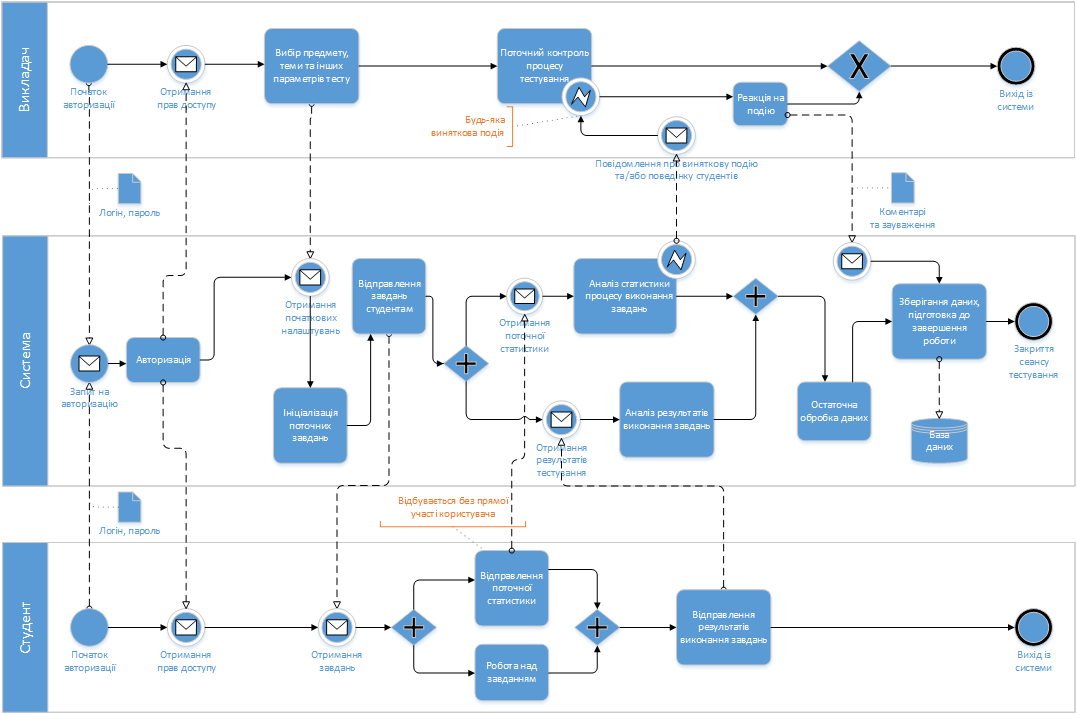
\includegraphics[height=28em,angle=-90]{images/bpmn_tests.png}
    \caption{BPMN-діаграма процесу проміжної перевірки знань,
    побудована на базі підрозділу \ref{section:precedences}}
    \label{fig:bpmn_tests}
\end{figure}

Користувачам потрібно спочатку авторизуватися, після чого студенти зможуть
отримувати завдання для виконання від відповідного сервера (сервіс видачі даних
для тестування), а викладачі зможуть отримувати від системи результати і ряд
рекомендацій щодо оцінювання.

Сервіс видачі даних орієнтується на ряд правил, серед яких частота користування
даними, використані дані в конкретній групі студентів, рівень знань конкретного
студента, рівень складності завдань тощо.
Правила націлені на покращення об’єктивності оцінювання.

Сервіс обробки результатів тестування опрацьовує результати кожного оцінювання.
При цьому відбувається як перевірка правильності виконання роботи, так і збір
різного роду статистики (час виконання як всього завдання так і окремих
підзавдань, кількість виправлень тощо), на основі якої система може
порекомендувати викладачу подальші дії: провести повторне тестування
конкретного студента, провести усне опитування (якщо студент не викликає довіри
протягом декількох спроб), змінити складність завдань або взагалі
переробити/видалити завдання.

Також можна розбити викладачів на декілька рівнів ієрархії відповідальності, де
інформація про оцінювання викладачами нижчих рівнів буде передаватися викладачам
вищих рівнів ієрархії.

Система не орієнтується на конкретний тип даних, тому можуть використовуватись
як прості тести з набором готових відповідей, так і завдання, де необхідно
написати текст пояснення, код програми, намалювати контур, побудувати діаграму
тощо.

Розглянемо схему з рис. \ref{fig:bpmn_teachers}.
Вона описує поведінку системи в режимі функціонування система-викладач.
Опустивши деталі авторизування користувачів, будемо вважати, що певну кількість
тестів успішно завершено (є тестову вибірку) і система має дані для роботи.

\begin{figure}[b!]
    \center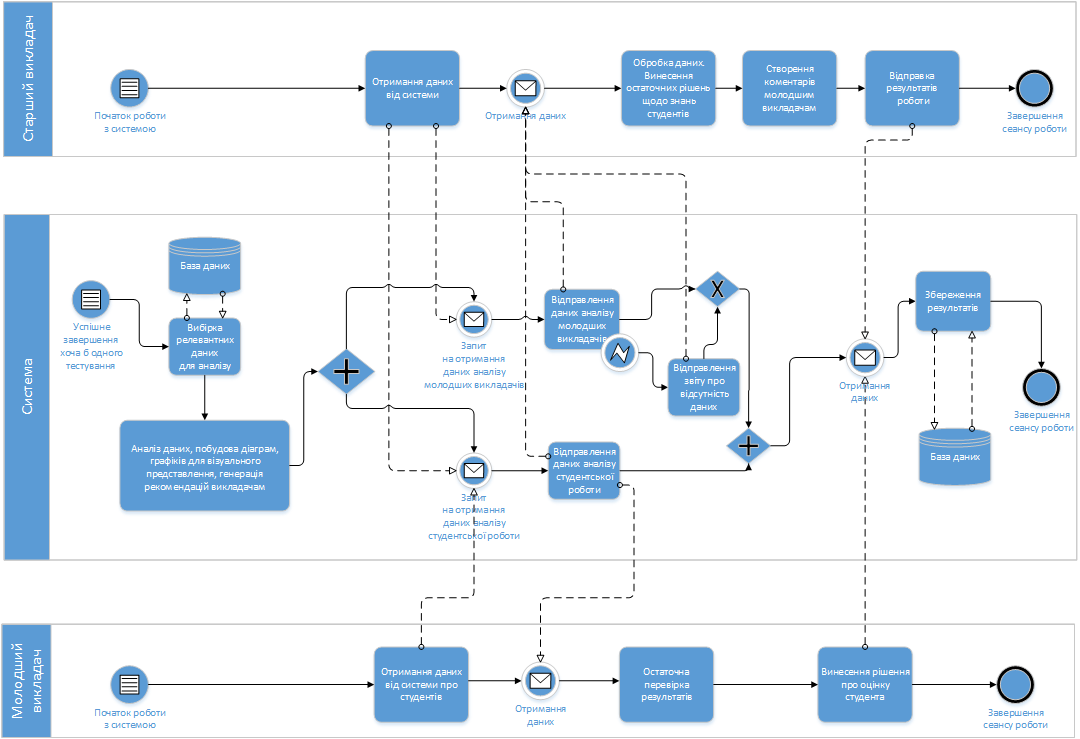
\includegraphics[height=30em,angle=-90]{images/bpmn_teachers.png}
    \caption{BPMN-діаграма процесу взаємодії викладачів і системи}
    \label{fig:bpmn_teachers}
\end{figure}

За таких початкових умов викладачі, що мають доступ до даних конкретного
курсу і групи, можуть продивлятися успішність студентів та аналізувати
статистику процесу тестування, що представлена наглядно.
На основі доступних даних викладач може змінювати оцінку студенту та
приймати рішення щодо подальшого оцінювання.

При реалізації системи онлайн тестування, тобто, в таких умовах, де студент може
здавати завдання з будь-якого місця, є доцільним реалізувати можливість
викладачу надати новий блок завдань студенту та відправити йому
повідомлення зі своїм рішенням --- в тому числі про необхідність усної здачі.

Крім того, викладач вищого рівня може контролювати оцінювання викладачів
нижчого. Наприклад, наскільки швидко завдання остаточно перевірені, наскільки
об’єктивне оцінювання та багато іншого.

Як було сказано у вступі, дана частина системи є однієї із найважливіших, бо
саме вона є базою для ідеї покращення об’єктивності навчання шляхом глибокого
аналізу різноманітних даних.


\chapter*{Висновки}
\addcontentsline{toc}{chapter}{Висновки}
% Крутая работа, заслуживающая наивысший балл, президентскую стипендию
% и отпуск на год.

Під час практики було розроблено базову концепцю майбутньої системи,
проаналізовано кілька готових рішень та фреймворків для розробки експертних
систем, а також були створені базові вимоги до системи,
проведено аналіз проблеми автоматизації навчання та створено ряд ідей щодо
його покращення.
З використанням даних ідей буде створено реальну систему покращення навчання з
мінімальними затратами часу та коштів.

З приводу вибору мови програмування, на якій буде реалізовано проект: JVM має
великий набір бібліотек і більш широке коло розробників, але Erlang націлений
на створення розподілених систем з високими вимогами до безпеки, а перевірка
часом і достатня кількість готових систем, що працюють роками, дозволяють
йому бути серйозним конкурентом іншим платформам у сфері розподілених
обчислень.

Також було вирішено, які галузі математики потрібні для досягнення поставленої
мети --- побудови моделей для максимально об’єктивного оцінювання, що означає
захист достовірності отримуваної від студентів інформації.

Маємо плани на світле майбутнє, є засоби, знання, ідеї щодо їх реалізації ---
залишилося з користю витратити наданий час.

Ідея є дійсно актуальною та варта реалізації.

\clearpage

\renewcommand\bibname{Перелік посилань}
\bibliography{../common/bibliography.bib}
% Workaround. Try to make two-paged bibliography
\addcontentsline{toc}{chapter}{Перелік посилань}

\end{document}
